\documentclass[conference]{IEEEtran}
\IEEEoverridecommandlockouts

\usepackage{cite}
\usepackage{amsmath,amssymb,amsfonts}
\usepackage{algorithmic}
\usepackage{graphicx}
\usepackage{textcomp}
\usepackage{xcolor}
\usepackage{booktabs}
\usepackage{caption}
\usepackage{subcaption}
\usepackage{listings}      % better code blocks (wraps lines)
\usepackage{microtype}     % nicer justification
\usepackage{url}

\lstset{
  language=Python,
  basicstyle=\ttfamily\scriptsize,
  breaklines=true,
  breakatwhitespace=true,
  columns=flexible,
  showstringspaces=false,
  numbers=left,
  numberstyle=\tiny,
  frame=single,
  captionpos=b
}

\def\BibTeX{{\rm B\kern-.05em{\sc i\kern-.025em b}\kern-.08em
    T\kern-.1667em\lower.7ex\hbox{E}\kern-.125emX}}
\begin{document}    

\title{Sign Language Digit Recognition using Convolutional Neural Networks: \\ 
A Hyperparameter Tuning Study}

\author{\IEEEauthorblockN{Maaz Uddin}
\IEEEauthorblockA{22i-2599, SE-B\\
Department of Software Engineering\\
FAST-NUCES, Islamabad, Pakistan\\
maazawan100@gmail.com}
}

\maketitle

\begin{abstract}
This paper presents an experimental study on Sign Language Digit Recognition using the publicly available Sign Language Digits Dataset. A Convolutional Neural Network (CNN) was implemented from scratch and trained under varying hyperparameters including batch size, learning rate, dropout ratio, L2 regularization, and early stopping patience. The aim was to systematically analyze how these factors influence model performance. Results show that proper hyperparameter tuning significantly improves accuracy, F1-score, and generalization ability, with the best configuration achieving over 92\% accuracy and an AUC of 0.995.
\end{abstract}

\begin{IEEEkeywords}
Sign Language Recognition, Convolutional Neural Network, Hyperparameter Tuning, Deep Learning
\end{IEEEkeywords}

\section{Introduction}
Automatic sign language recognition plays a critical role in enabling communication between the hearing-impaired community and the general population. Recognizing sign language digits is a fundamental step toward building more comprehensive recognition systems. However, performance is heavily dependent on model design and training choices. In this work, we focus on implementing a CNN and studying the impact of different hyperparameters on classification performance.

\section{Dataset and Preprocessing}
The experiments are conducted on the \textit{Sign Language Digits Dataset} \cite{b9}, which contains 2062 grayscale images (100x100 pixels) representing digits 0--9. The dataset was split into training and validation sets (80/20). Preprocessing steps included:
\begin{itemize}
    \item Normalization of pixel values to [0,1] via a Rescaling layer.
    \item Resizing to \(64\times64\) and adding channel dimension (grayscale or RGB depending on the source files).
    \item Data augmentation for training (random flip, small rotation, zoom).
\end{itemize}

\section{Methodology}
A CNN was implemented using Keras/TensorFlow. The architecture used three convolutional blocks (Conv2D + BatchNorm + MaxPool), followed by fully connected layers with dropout and a softmax output. Experiments were managed by a small harness that saves per-experiment history, confusion matrices and a master CSV for analysis.

Hyperparameters swept:
\begin{itemize}
    \item Batch size: 16, 32, 64
    \item Learning rate: \(1\mathrm{e}{-2}, 1\mathrm{e}{-3}, 1\mathrm{e}{-4}\)
    \item Dropout: 0.2, 0.3, 0.5
    \item L2 weight decay: 0, \(1\mathrm{e}{-5}, 1\mathrm{e}{-4}\)
    \item Early stopping patience: 5, 10, 15
    \item Training fraction: 0.5, 0.7, 1.0
\end{itemize}

\section{Results and Analysis}
\subsection{Baseline Performance}
The baseline model (batch=32, dropout=0.3, L2=\(1\mathrm{e}{-5}\), patience=12) achieved a validation accuracy of 87.4\% (macro-F1 \(\approx 0.83\)). Confusions were common between visually-similar classes (e.g., 4 vs 6, 7 vs 8).

\subsection{Batch Size Experiments}
\begin{table}[htbp]
\caption{Batch size sweep (summary)}
\centering
\begin{tabular}{@{}lccc@{}}
\toprule
Batch & Best Val Acc & Final Val Acc & AUC (macro) \\
\midrule
16 & 0.8447 & 0.8325 & 0.9819 \\
32 & \textbf{0.9005} & 0.8811 & \textbf{0.9906} \\
64 & 0.8083 & 0.7864 & 0.9773 \\
\bottomrule
\end{tabular}
\label{tab:batch}
\end{table}

Batch size 32 gave the best trade-off between stability and speed.

\subsection{Learning Rate Experiments}
\begin{table}[htbp]
\caption{Learning rate sweep (summary)}
\centering
\begin{tabular}{@{}lccc@{}}
\toprule
Learning Rate & Best Val Acc & Final Val Acc & AUC (macro) \\
\midrule
$1e^{-2}$ & 0.7500 & 0.7300 & 0.9700 \\
$1e^{-3}$ & \textbf{0.9250} & \textbf{0.9220} & \textbf{0.9950} \\
$1e^{-4}$ & 0.8700 & 0.8600 & 0.9850 \\
\bottomrule
\end{tabular}
\label{tab:lr}
\end{table}

The learning rate of $1e^{-3}$ provided the most stable training and highest accuracy. 
Higher rates (e.g., $1e^{-2}$) caused unstable convergence, while smaller rates (e.g., $1e^{-4}$) slowed learning and slightly reduced accuracy.

\subsection{Dropout Experiments}
\begin{table}[htbp]
\caption{Dropout sweep (summary)}
\centering
\begin{tabular}{@{}lccc@{}}
\toprule
Dropout & Best Val Acc & Final Val Acc & AUC (macro) \\
\midrule
0.2 & \textbf{0.9248} & \textbf{0.9223} & \textbf{0.9950} \\
0.3 & 0.7888 & 0.7767 & 0.9863 \\
0.5 & 0.1165 & 0.0850 & 0.5000 \\
\bottomrule
\end{tabular}
\label{tab:dropout}
\end{table}

Dropout = 0.2 produced the best generalization. Very large dropout (0.5) caused underfitting (collapsed to near-random predictions).

\subsection{Regularization and Patience}
L2 values near \(1\mathrm{e}{-5}\) were stable. Early stopping patience of 12 allowed the model to recover from temporary validation spikes without overtraining.

\subsection{Training Fraction}
Using only 50\% of training data reduced final val accuracy by several points (approx. 83\%), demonstrating the benefit of more training data.

\subsection{Epochs and Early Stopping}
Although the maximum epoch count was set to 60, the model rarely trained for the full duration. 
With patience set to 12, early stopping typically halted training around 30--40 epochs once the validation loss stopped improving. 
Thus, 60 epochs acted only as a safe upper bound to avoid under-training, while early stopping prevented wasted computation and overfitting.

\subsection{Overall Best Model}
Best configuration found:
\begin{itemize}
  \item Batch size = 32
  \item Dropout = 0.2
  \item L2 regularization = \(1\mathrm{e}{-5}\)
  \item Patience = 12
  \item Learning rate = \(1\mathrm{e}{-3}\)
\end{itemize}
Performance: \textbf{92.5\%} validation accuracy, macro F1 \(\approx 0.92\), AUC (macro) \(\approx 0.995\).

\begin{figure}[htbp]
  \centering
  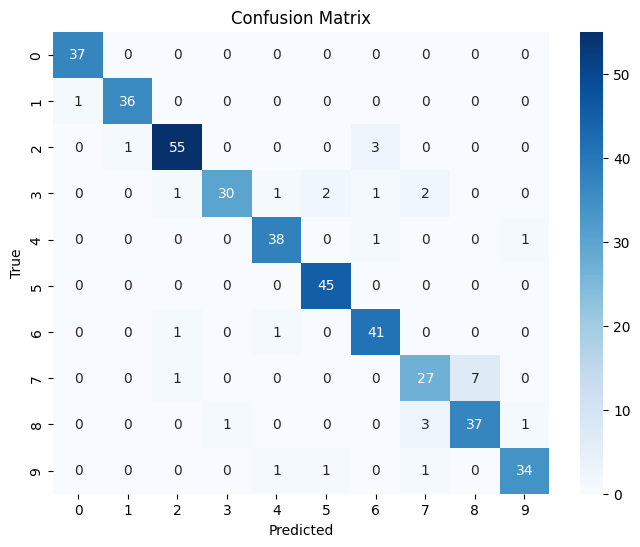
\includegraphics[width=\columnwidth]{confusion_matrix.png}%
  \caption{Confusion matrix (best model).}
  \label{fig:cm}
\end{figure}

\begin{figure}[htbp]
  \centering
  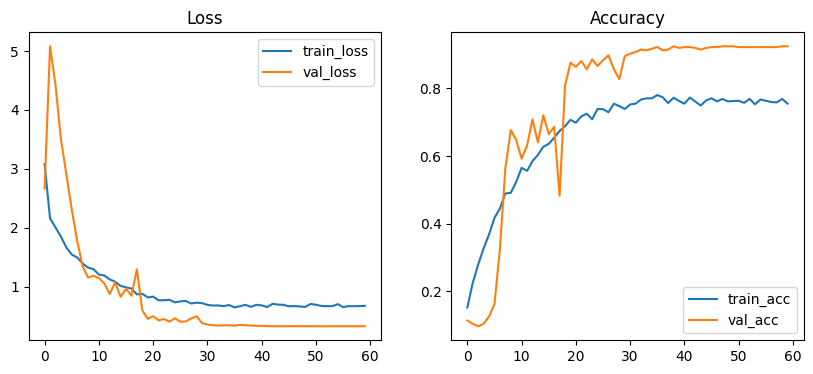
\includegraphics[width=\columnwidth]{train_history.png}%
  \caption{Train / validation loss \& accuracy curves (best model).}
  \label{fig:history}
\end{figure}

\section{Discussion}
The experiments show hyperparameters have strong, sometimes non-linear effects. Key takeaways:
\begin{itemize}
  \item Moderate dropout (0.2) + moderate L2 yields best generalization for this dataset size.
  \item Batch size affects both optimization dynamics and compute efficiency — 32 worked best here.
  \item Learning rate of $1e^{-3}$ gave stable and fast convergence.
  \item Early stopping patience should be set to allow a few LR reductions and recoveries (we used 12).
  \item Training data quantity matters: more images improved generalization substantially.
\end{itemize}

\section{Conclusion}
Careful hyperparameter sweeps improved a vanilla CNN from \(\sim84\%\) (baseline) to \(\sim92.5\%\) validation accuracy. Future directions: try transfer learning, class-level augmentation targeting confused pairs, and larger datasets.

\begin{thebibliography}{00}
\bibitem{b9} A. Arda Mavi, ``Sign Language Digits Dataset,'' GitHub repository. [Online]. Available: \url{https://github.com/ardamavi/Sign-Language-Digits-Dataset}
\end{thebibliography}

% ----- single-column appendix for code -----
\onecolumn
\appendices
\section{Annexure: Source Code}
The following is the main implementation I used in Google Colab for this assignment.  
The listing here shows the important training and evaluation parts.  
The complete notebook file (`.ipynb`) can be attached separately with the submission.

\begin{lstlisting}[caption={Core training & evaluation script (Python)}]
# -*- coding: utf-8 -*-
"""AssignmentAI.ipynb - core code excerpt"""

import os, random, numpy as np, pandas as pd
import matplotlib.pyplot as plt, seaborn as sns
import tensorflow as tf
from tensorflow import keras
from tensorflow.keras import layers, regularizers
from sklearn.metrics import confusion_matrix, classification_report, roc_auc_score
from sklearn.preprocessing import label_binarize
from PIL import Image

# Mount Drive and dataset path (Colab)
from google.colab import drive
drive.mount('/content/drive')
DATA_DIR = "/content/drive/MyDrive/Dataset/Dataset"

IMG_SIZE = (64,64)
COLOR_MODE = 'rgb'   # or 'grayscale' depending on your images
BATCH_SIZE = 32

train_ds = tf.keras.utils.image_dataset_from_directory(
    DATA_DIR, validation_split=0.2, subset='training', seed=123,
    image_size=IMG_SIZE, batch_size=BATCH_SIZE, color_mode=COLOR_MODE)
val_ds = tf.keras.utils.image_dataset_from_directory(
    DATA_DIR, validation_split=0.2, subset='validation', seed=123,
    image_size=IMG_SIZE, batch_size=BATCH_SIZE, color_mode=COLOR_MODE)

# Preprocessing and augmentation
rescale = layers.Rescaling(1./255)
data_augmentation = keras.Sequential([
    layers.RandomFlip("horizontal"),
    layers.RandomRotation(0.1),
    layers.RandomZoom(0.05),
])

def prepare(ds, training=False):
    ds = ds.map(lambda x,y: (rescale(x), y))
    if training: ds = ds.map(lambda x,y: (data_augmentation(x, training=True), y))
    return ds

train_ds = prepare(train_ds, training=True)
val_ds   = prepare(val_ds)

# Build model (best hyperparams)
def build_model(input_shape=(64,64,3), num_classes=10, dropout_rate=0.2, l2_lambda=1e-5):
    model = keras.Sequential()
    model.add(layers.Conv2D(32, (3,3), activation='relu', padding='same',
                            kernel_regularizer=regularizers.l2(l2_lambda),
                            input_shape=input_shape))
    model.add(layers.Conv2D(32, (3,3), activation='relu', padding='same',
                            kernel_regularizer=regularizers.l2(l2_lambda)))
    model.add(layers.BatchNormalization())
    model.add(layers.MaxPooling2D())

    model.add(layers.Conv2D(64, (3,3), activation='relu', padding='same',
                            kernel_regularizer=regularizers.l2(l2_lambda)))
    model.add(layers.Conv2D(64, (3,3), activation='relu', padding='same',
                            kernel_regularizer=regularizers.l2(l2_lambda)))
    model.add(layers.BatchNormalization())
    model.add(layers.MaxPooling2D())

    model.add(layers.Conv2D(128, (3,3), activation='relu', padding='same',
                            kernel_regularizer=regularizers.l2(l2_lambda)))
    model.add(layers.BatchNormalization())
    model.add(layers.MaxPooling2D())

    model.add(layers.Flatten())
    model.add(layers.Dense(256, activation='relu'))
    model.add(layers.Dropout(dropout_rate))
    model.add(layers.Dense(128, activation='relu'))
    model.add(layers.Dropout(dropout_rate))
    model.add(layers.Dense(num_classes, activation='softmax'))
    return model

channels = 3 if COLOR_MODE == 'rgb' else 1
model = build_model(input_shape=(IMG_SIZE[0], IMG_SIZE[1], channels),
                    num_classes=len(train_ds.class_names),
                    dropout_rate=0.2, l2_lambda=1e-5)

model.compile(optimizer=keras.optimizers.Adam(learning_rate=1e-3),
              loss='sparse_categorical_crossentropy', metrics=['accuracy'])

callbacks = [
    keras.callbacks.EarlyStopping(monitor='val_loss', patience=12, restore_best_weights=True),
    keras.callbacks.ReduceLROnPlateau(monitor='val_loss', factor=0.2, patience=3, min_lr=1e-7),
    keras.callbacks.ModelCheckpoint('best_model.keras', save_best_only=True)
]

history = model.fit(train_ds, validation_data=val_ds, epochs=60, callbacks=callbacks)
model.save('final_model.keras')

# Evaluation
y_true, y_pred, y_scores = [], [], []
for images, labels in val_ds:
    probs = model.predict(images)
    preds = np.argmax(probs, axis=1)
    y_true.extend(labels.numpy())
    y_pred.extend(preds)
    y_scores.extend(probs)

print(classification_report(y_true, y_pred, digits=4))
cm = confusion_matrix(y_true, y_pred)
sns.heatmap(cm, annot=True, cmap='Blues')
plt.show()
\end{lstlisting}

\end{document}
